\documentclass[tikz,border=3mm]{standalone}
\usepackage{booktabs}

\begin{document}

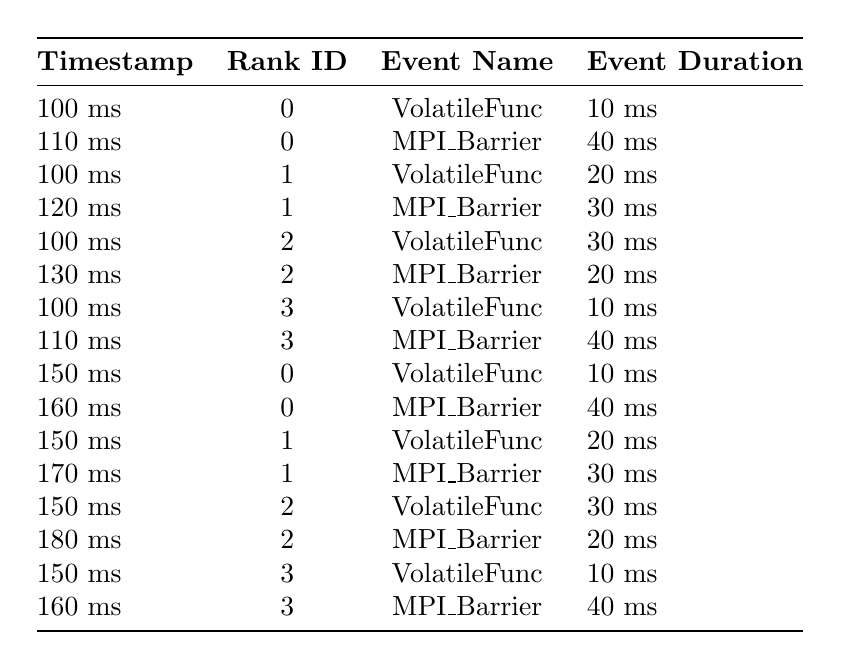
\begin{tikzpicture}

  \node[anchor=north west] at (0, 0) {
    \begin{tabular}
      {@{}lccl@{}}
      \toprule
      \textbf{Timestamp} & \textbf{Rank ID} & \textbf{Event Name} & \textbf{Event Duration} \\
      \midrule
      100 ms             & 0                & VolatileFunc        & 10 ms                   \\
      110 ms             & 0                & MPI\_Barrier        & 40 ms                   \\
      100 ms             & 1                & VolatileFunc        & 20 ms                   \\
      120 ms             & 1                & MPI\_Barrier        & 30 ms                   \\
      100 ms             & 2                & VolatileFunc        & 30 ms                   \\
      130 ms             & 2                & MPI\_Barrier        & 20 ms                   \\
      100 ms             & 3                & VolatileFunc        & 10 ms                   \\
      110 ms             & 3                & MPI\_Barrier        & 40 ms                   \\
      150 ms             & 0                & VolatileFunc        & 10 ms                   \\
      160 ms             & 0                & MPI\_Barrier        & 40 ms                   \\
      150 ms             & 1                & VolatileFunc        & 20 ms                   \\
      170 ms             & 1                & MPI\_Barrier        & 30 ms                   \\
      150 ms             & 2                & VolatileFunc        & 30 ms                   \\
      180 ms             & 2                & MPI\_Barrier        & 20 ms                   \\
      150 ms             & 3                & VolatileFunc        & 10 ms                   \\
      160 ms             & 3                & MPI\_Barrier        & 40 ms                   \\
      \bottomrule
    \end{tabular}
  };

\end{tikzpicture}

\end{document}